\section{Surrogate Models Overview}

Large-scale computational models are crucial tools to analyze complex systems. When coupled with uncertainty quantification and optimization methods, the resulting computational expense becomes intractable. In order to face the computational burden, surface approximation methods, black box models, or surrogate models are commonly used. FOQUS provides a selection of surrogate modeling tools all using a similar work-flow. This section provides an overview of the surrogate modeling features and capabilities. The details of each tool are provided in the tutorial sections.

The following surrogate modeling tools are currently available:
\begin{itemize}
	\item ACOSSO -- Adaptive COmponent Selection and Shrinkage Operator is a regularization method for simultaneous model fitting and variable selection based in nonparametric regression methods. ACCOSSO is suitable for approximating models  with
     many inputs and no sharp changes.
	\item ALAMO -- Automated Learning of Algebraic Models for Optimization generates algebraic models from data sets. These surrogate models are ideal for equation
     oriented optimization problems (which are
     easily differentiable), such as super structure optimization.
	\item BSS-ANOVA -- Bayesian Smoothing Spline Analysis of Variance is a method similar to ACOSSO.
	\item iREVEAL -- Surrogate models for CFD simulations using Kriging or
     Neural Networks. It contains special features specifically designed
     for working with CFDs. 
\end{itemize}

\subsection{Data Selection}

The \bu{Data} tab allows the selection of training data to be used to generate a surrogate model (Figure \ref{fig.surrogate.data}). If the session is associated with a flowsheet data (results from a single flowsheet run, optimization runs, or UQ samples), then the flowsheet data is available to be the training data and the table will be populated accordingly.

\begin{figure}[H]
	\begin{center}
		\includegraphics[scale=0.55]{Chapt_surrogates/figs/data_form}
		\caption{Surrogate Data Form}
		\label{fig.surrogate.data}
	\end{center}
\end{figure}
\begin{enumerate}
	\item \bu{Run} the surrogate modeling method.
	\item \bu{Stop} the surrogate modeling method.
	\item \bu{Surrogate modeling tool} enables the user to select the desired surrogate modeling tool from the \textbf{\underline{Tool}} drop-down list.
	\item \bu{Description} of the selected surrogate method.
	\item \bu{Add Samples} enables the user to generate new training data using a model specified in the flowsheet or an emulator (i.e., a basic response surface provided as part of the UQ module).
	\item \bu{Flowsheet Results} are summarized below.
	\item The data table has a \bu{Menu} drop-down list that contains display, import/export, and edit commands. 
	\item Select a data filter from the \bu{Current Filter} drop-down for current data display.
	\item Add or edit new data filters from \bu{Edit Filters}. This dialog is shown in Figure \ref{fig.filter.1.result}.
	\item The \bu{Display} table displays the results of flowsheet evaluations stored in the FOQUS session file. The columns are:
	\begin{itemize}
		\item \bu{SetName} is a name assigned to samples. This is typically
        equivalent to one UQ sample run or one optimization run.
		\item \bu{ResultName} is a string representing a result name.
		\item \bu{Error} is the simulation result status; 0 indicates success, other numbers represent an error. A column for each node displays the error status of each node.
		\item \bu{Time} displays the time when the result was stored.
		\item \bu{Elapsed Time} describes how long a result took to calculate. 
		\item \bu{Tags} enables a list of string labels to be applied to results. This could be used to mark results to be used for a particular purpose such as model validation.
		\item The remaining columns display the input and output variables.
	\end{itemize}
\end{enumerate}

Filters can be used to select data. See Section
\ref{tutorials.fs.data} for more information on creating filters to the results.
The ``All'' and ``None'' filters are available by default. These can be
used, for example, to assign all the data as a training set, or to split
the data into a separate training set and a test set.

\subsection{Variables}

The \bu{Variables} section is illustrated in Figure
\ref{fig.surrogate.vars}.  This section allows selection of input and
output variables used in a surrogate model.  Some surrogate methods such as ALAMO may generate and run additional samples while building surrogates.
The \textbf{\underline{Min/Max}} columns provide bounds on the variables. Selecting the checkbox next to the variable \textbf{\underline{Name}} indicates that it should be included in the surrogate generation. Failure to select a checkbox for any variables will result in error during surrogate generation.

\begin{figure}[H]
	\begin{center}
		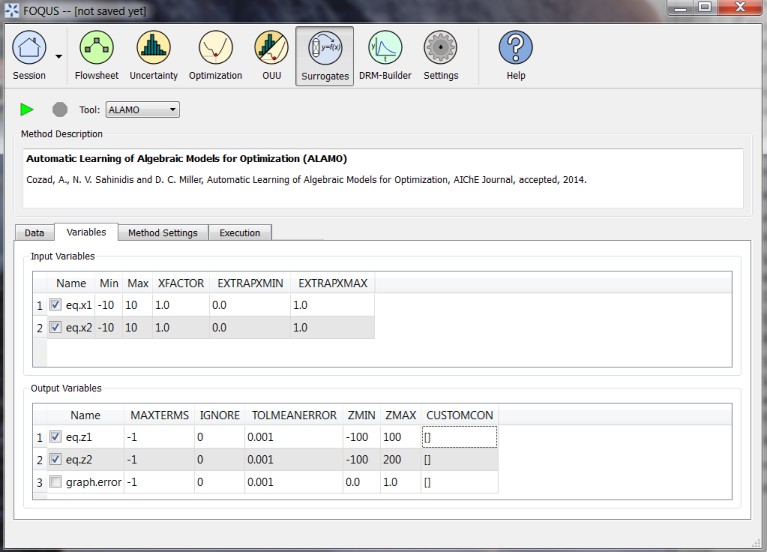
\includegraphics[scale=0.55]{Chapt_surrogates/figs/vars}
		\caption{Surrogate Variable Selection}
		\label{fig.surrogate.vars}
	\end{center}
\end{figure}

\subsection{Method Settings}

The \bu{Method Settings} table is illustrated in Figure
\ref{fig.surrogate.settings}.  The settings available in this table depend on the surrogate tool. A description of each setting is provided in the third column of the table.
%The figure is labeled "Surrogate Settings", but this section is labeled "Method Settings". Should they match or be changed to "Surrogate Models, Method Settings"?
\begin{figure}[H]
	\begin{center}
		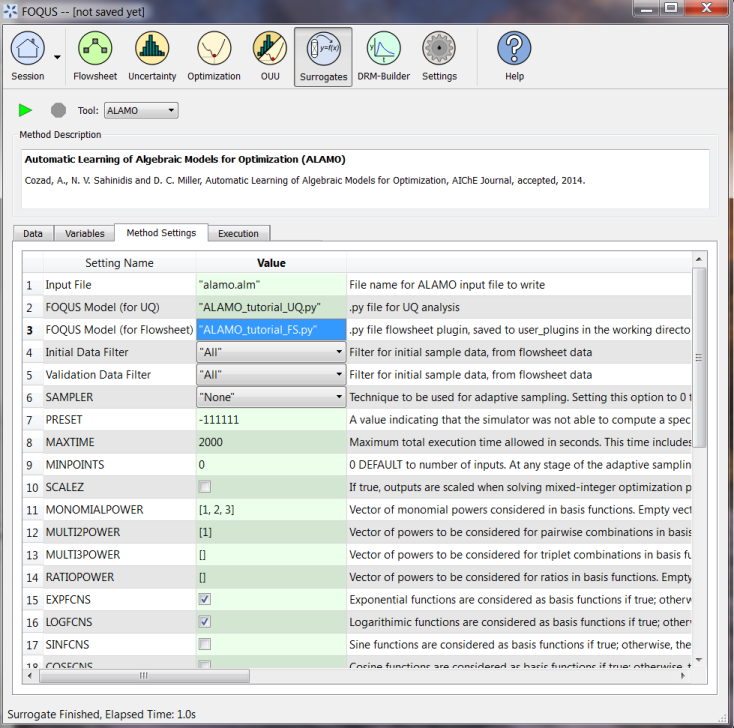
\includegraphics[scale=0.55]{Chapt_surrogates/figs/settings}
		\caption{Surrogate Settings}
		\label{fig.surrogate.settings}
	\end{center}
\end{figure}

\subsection{Execution}

Clicking \bu{Run} starts the surrogate model building process.  The
execution monitor displays after \bu{Run} is clicked (see Figure
\ref{fig.surrogate.monitor}). The execution monitor displays the status of the surrogate build. The messages displayed depends on the surrogate tool.

\begin{figure}[H]
	\begin{center}
		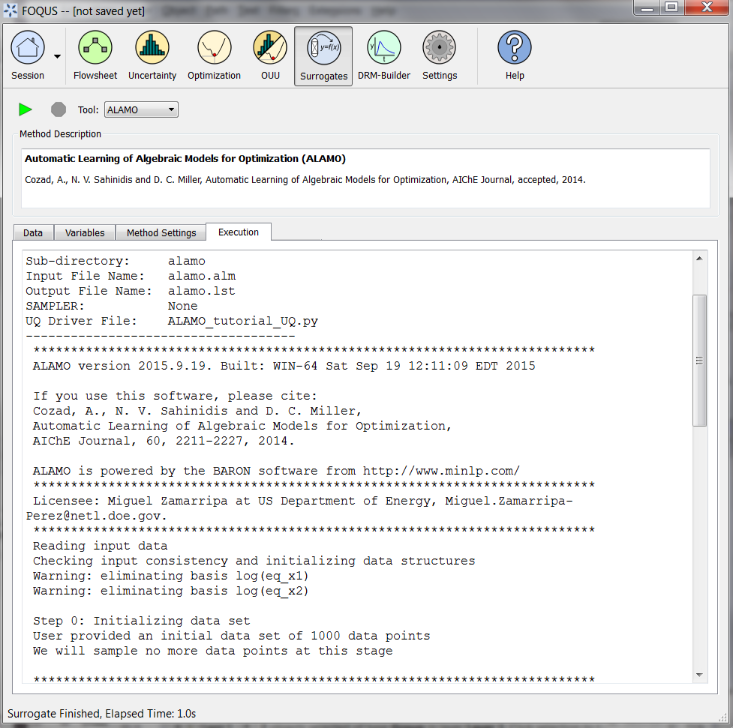
\includegraphics[scale=0.55]{Chapt_surrogates/figs/monitor}
		\caption{Surrogate Status Monitor}
		\label{fig.surrogate.monitor}
	\end{center}
\end{figure}

%\subsection{Results}
After a successful execution and model building, the results are displayed. Note that in this case, the surrogate modeling tool ends with an error, the errors are displayed in this window. After surrogate generation completes, one or two Python files will be generated depending on the tool. Each tool generates a file that encodes the surrogate model as a general Python script that can be used to evaluate output values for UQ analyses within the UQ module. The other file, if available, is a FOQUS flowsheet plugin model that allows the surrogate to be run in a FOQUS flowsheet. The next version of FOQUS will generate a FOQUS flowsheet plugin model (i.e., the second file) for all surrogate tools.

